\documentclass[10pt, oneside]{article}
\usepackage[letterpaper, margin=1in]{geometry}
%\usepackage[parfill]{parskip}    		% Activate to begin paragraphs with an empty line rather than an indent
\usepackage{graphicx}
\usepackage{amssymb}
\usepackage[style=numeric,firstinits=true,backend=bibtex]{biblatex}
\addbibresource{main}     %Adds the bib file (bib-database)
\usepackage{wrapfig}
\usepackage{algorithm}
\usepackage{algpseudocode}      % for writing pseudocode
\usepackage{amsmath}
\usepackage{amsfonts}
\usepackage{url}
% \usepackage{tikz}              % for drawing superb diagrams, use omni-graffle or yEd
% \usetikzlibrary{calc,shapes.multipart,chains,arrows}
\usepackage{graphicx}
\usepackage{nameref}            % Cross-referencing to include the name of the section, 
                                % rather than just the number or page

% \usepackage{adjustbox}          %Adjustments like in "includegraphics" options
\usepackage{framed}             % Create framed, shaded, or differently highlighted 
                                % regions that can break across pages
\usepackage[all]{xy}
\usepackage{txfonts,pxfonts}    %additional fonts: for more symbols
\usepackage{bm}
\usepackage{enumerate}          %gives the enumerate environment an optional argument
                                % which determines the style in which the counter is 
                                % printed
\usepackage{subfigure}          %for sub figures
\usepackage[linktoc=all]{hyperref}
\usepackage{enumitem}
\usepackage{multirow}
\setlength{\parskip}{.25ex plus1mm minus1mm}
% ----------------------------------------
%  Nice code using inconsolata font
% ----------------------------------------

%\usepackage{listings}
\usepackage{xcolor}

% Code listing stuff
\usepackage{listings}
\usepackage[T1]{fontenc}
\usepackage[utf8]{inputenc}
\usepackage[scaled=0.8]{beramono}
\usepackage{amsmath}
\usepackage{amsfonts}
\usepackage{amssymb}
\definecolor{light-gray}{gray}{0.45}
\definecolor{dark-green}{rgb}{0.0,0.34,0.25}

\lstset { language=Python }

\lstset { 
	% Basic formatting
	basicstyle=\ttfamily\footnotesize,
	keywordstyle=\color{blue}\ttfamily\bfseries,
	commentstyle=\color{light-gray}\ttfamily\itshape,
	breaklines=true,
	escapechar=\%,
	showspaces=false,
	captionpos=b,
	%abovecaptionskip=\medskipamount,
	%belowskip=-2em,
	% Line numbering
	numbers=left,
	xleftmargin=3.6em,
	framexleftmargin=1.5em,
	numberstyle=\color{light-gray},
	firstnumber=1,
	numberfirstline=true
}


%\usepackage{fontspec}
%\setmonofont{Consolas}

%\lstdefinelanguage{ds2}{
%  morekeywords={
%    world, machine, agents, compute, %
%    agents-bandwidth, agents-reactions , %
%    level, parent, sync, async, send, broadcast,%
%    reactions, sender,
%    schedule, function,%
%    on-join, on-rejoin, on-leave, on-start, on-demise, on-link-failed,%
%    abstract,case,catch,class,def,%
%    do,else,extends,false,final,finally,%
%    for,if,implicit,import,match,mixin,%
%    new,null,object,override,package,%
%    private,protected,requires,return,sealed,%
%    super,this,throw,trait,true,try,%
%    type,val,var,while,with,yield},
%  otherkeywords={!,:,=>,<-,<\%,<:,>:,\#,@},
%  sensitive=true,
%  morecomment=[l]{//},
%  morecomment=[n]{/*}{*/},
%  morestring=[b]",
%  morestring=[b]',
%  morestring=[b]"""
%}
%
%\lstset{ %
%  postbreak=\raisebox{0ex}[0ex][0ex]{\ensuremath{\color{red}\hookrightarrow\space}}, % shows hook arrow and indents wrapped line 
%  backgroundcolor=\color{white},   % choose the background color; you must add \usepackage{color} or \usepackage{xcolor}
%  basicstyle=\tiny,        % the size of the fonts that are used for the code
%  breakatwhitespace=false,         % sets if automatic breaks should only happen at whitespace
%  breaklines=true,                 % sets automatic line breaking
%  captionpos=b,                    % sets the caption-position to bottom
%  commentstyle=\color{olive},    % comment style
%  deletekeywords={...},            % if you want to delete keywords from the given language
%  escapeinside={\%*}{*)},          % if you want to add LaTeX within your code
%  extendedchars=true,              % lets you use non-ASCII characters; for 8-bits encodings only, does not work with UTF-8
%  frame=single,	                   % adds a frame around the code
%  keepspaces=true,                 % keeps spaces in text, useful for keeping indentation of code (possibly needs columns=flexible)
%  keywordstyle=\color{blue},       % keyword style
%  language=ds2,                 % the language of the code
%  otherkeywords={*,...},           % if you want to add more keywords to the set
%  numbers=left,                    % where to put the line-numbers; possible values are (none, left, right)
%  numbersep=5pt,                   % how far the line-numbers are from the code
%  numberstyle=\tiny\color{gray}, % the style that is used for the line-numbers
%  rulecolor=\color{gray},         % if not set, the frame-color may be changed on line-breaks within not-black text (e.g. comments (green here))
%  showspaces=false,                % show spaces everywhere adding particular underscores; it overrides 'showstringspaces'
%  showstringspaces=false,          % underline spaces within strings only
%  showtabs=false,                  % show tabs within strings adding particular underscores
%  stepnumber=2,                    % the step between two line-numbers. If it's 1, each line will be numbered
%  stringstyle=\color{red},     % string literal style
%  tabsize=2,	                   % sets default tabsize to 2 spaces
%  title=\lstname,                   % show the filename of files included with \lstinputlisting; also try caption instead of title
%}

% ----------------------------------------

% \raggedbottom % less spacing between items 

% Recommended, but optional, packages for figures and better typesetting:
\usepackage{microtype}
\usepackage{graphicx}
\usepackage{subfigure}
\usepackage{booktabs} % for professional tables
\usepackage{tabularx}
\usepackage{upgreek}
\usepackage{comment}
\usepackage{amsmath,array,graphicx}

\usepackage{tabularx}
\usepackage{multirow}
\usepackage{graphicx}
\usepackage{algorithm}
%\usepackage[noend]{algpseudocode}
\usepackage[colorinlistoftodos]{todonotes}
%\usepackage{algorithm,algpseudocode}
\usepackage{upgreek}

% hyperref makes hyperlinks in the resulting PDF.
% If your build breaks (sometimes temporarily if a hyperlink spans a page)
% please comment out the following usepackhttps://www.overleaf.com/project/5cedce0cdfbeaa5a7375b030age line and replace
% \usepackage{sysml2019} with \usepackage[nohyperref]{sysml2019} above.
%\usepackage{hyperref}

% Attempt to make hyperref and algorithmic work together better:
\newcommand{\theHalgorithm}{\arabic{algorithm}}

\newcommand{\argmin}{\operatornamewithlimits{argmin}}
\newcommand{\argmax}{\operatornamewithlimits{argmax}}
\newcommand{\bx}{{\bf x}}
\newcommand{\bs}{{\bf s}}
\newcommand{\bd}{{\bf d}}
\newcommand{\by}{{\bf y}}
\newcommand{\bw}{{\bf w}}
\newcommand{\bh}{{\bf h}}
\newcommand{\bb}{{\bf b}}
\newcommand{\bE}{{\bf E}}
\newcommand{\bH}{{\bf H}}
\newcommand{\bP}{{\bf P}}
\newcommand{\bC}{{\bf C}}
\newcommand{\bS}{{\bf S}}

% Code listing stuff
\usepackage{listings}
\usepackage[T1]{fontenc}
\usepackage[utf8]{inputenc}
\usepackage[scaled=0.8]{beramono}
\usepackage{amsmath}
\usepackage{amsfonts}
\usepackage{amssymb}
\usepackage{xcolor}
\usepackage{xspace}
\definecolor{light-gray}{gray}{0.45}
\definecolor{dark-green}{rgb}{0.0,0.34,0.25}

\title{\huge \textbf{Systems and Methods for Resource Efficient \\ and Reliable Neural Network Compression}}
%
\author{\\
        \\\huge \textbf{Dissertation Proposal} \\
        \\
        \\
        \\\huge \textbf{Candidate} \\
        \\
        \\\huge Vinu Joseph \\
        \\ \LARGE \texttt{vinu@cs.utah.edu}
        \\
        \\
        \\
        \\
        \\\huge \textbf{Committee}\\
        \\
        \\\huge Ganesh Gopalakrishnan \\
        \\\huge Aditya Bhaskara \\
        \\\huge Vivek Srikumar \\
        \\\huge Mary Hall \\
        \\\huge Michael Garland \\
        
        }
\date{}
%
%\date{\LARGE October 09, 2018 -- October 16, 2018}
%        
%
%\title{\textbf{PhD Written Qualifier Exam}
%\vspace{5ex}
%\\
%\underline{Examiners}
%\\ 
%Ganesh Gopalakrishnan
%\\
%Mary Hall
%\\
%Aditya Bhaskara
%\\
%Vivek Srikumar}
%%
%\author{\underline{Examinee}\\ Vinu Joseph\\{\texttt{vinu@cs.utah.edu}}}
%
%
\renewcommand*{\bibfont}{\footnotesize}
\lstset{basicstyle=\ttfamily,
escapeinside={||},
mathescape=true}
%
\newenvironment{blockquote}{\par\medskip\leftskip=4em\rightskip=2em\noindent\ignorespaces}{\par\medskip}
%
%\DeclareMathOperator*{\argmax}{arg\,max}
%\DeclareMathOperator*{\argmin}{arg\,min}
\newcommand{\norm}[1]{\left\lVert#1\right\rVert}
\newcommand{\algoName}[0]{\textsc{Condensa}\xspace}
%
\begin{document}
\maketitle
\newpage
\setcounter{tocdepth}{3}
\tableofcontents
\newpage

%\begin{refsection}
\section{Introduction}


Modern deep neural networks (DNNs) are complex,
and often contain millions of parameters spanning
dozens or even hundreds of layers~\cite{he2016deep,huang:2017}.
%
This complexity translates into substantial memory and runtime costs
on hardware platforms at all scales.
%
Recent work has demonstrated that DNNs are often over-provisioned and can be compressed without appreciable loss of accuracy.
Model compression can be used to
reduce both model memory footprint and inference latency using techniques such as
weight pruning~\cite{han2015learning,luo2017thinet},
quantization~\cite{gupta2015deep}, and low-rank
factorization~\cite{jaderberg2014speeding,denton2014exploiting}.
%
Unfortunately, the requirements of
different {\em compression contexts}---DNN structure,
target hardware platform, and the user's optimization objective---are often in conflict.
%
The recommended compression strategy for reducing inference latency
may be different from that required to reduce total memory footprint.
%
For example, in a Convolutional Neural Network (CNN),
reducing inference latency may require pruning filters to realize speedups on real hardware~\cite{li2016pruning}, while reducing memory footprint may be accomplished by zeroing out individual weights.
%
Similarly, even for the {\em same optimization objective},
say reducing inference latency, one may employ filter pruning for a CNN,
while pruning 2-D blocks of non-zero weights~\cite{gray:2017} for a
language modeling network such as Transformer~\cite{vaswani:2017},
since the latter has no convolutional layers.
%
Thus, it is crucial to enable convenient expression of 
alternative compression schemes, yet
none of today's model compression approaches help the designer
tailor compression schemes to their needs.


\begin{figure}[!h]
\centering
%\fbox{\rule{0pt}{2in} \rule{0.9\linewidth}{0pt}}
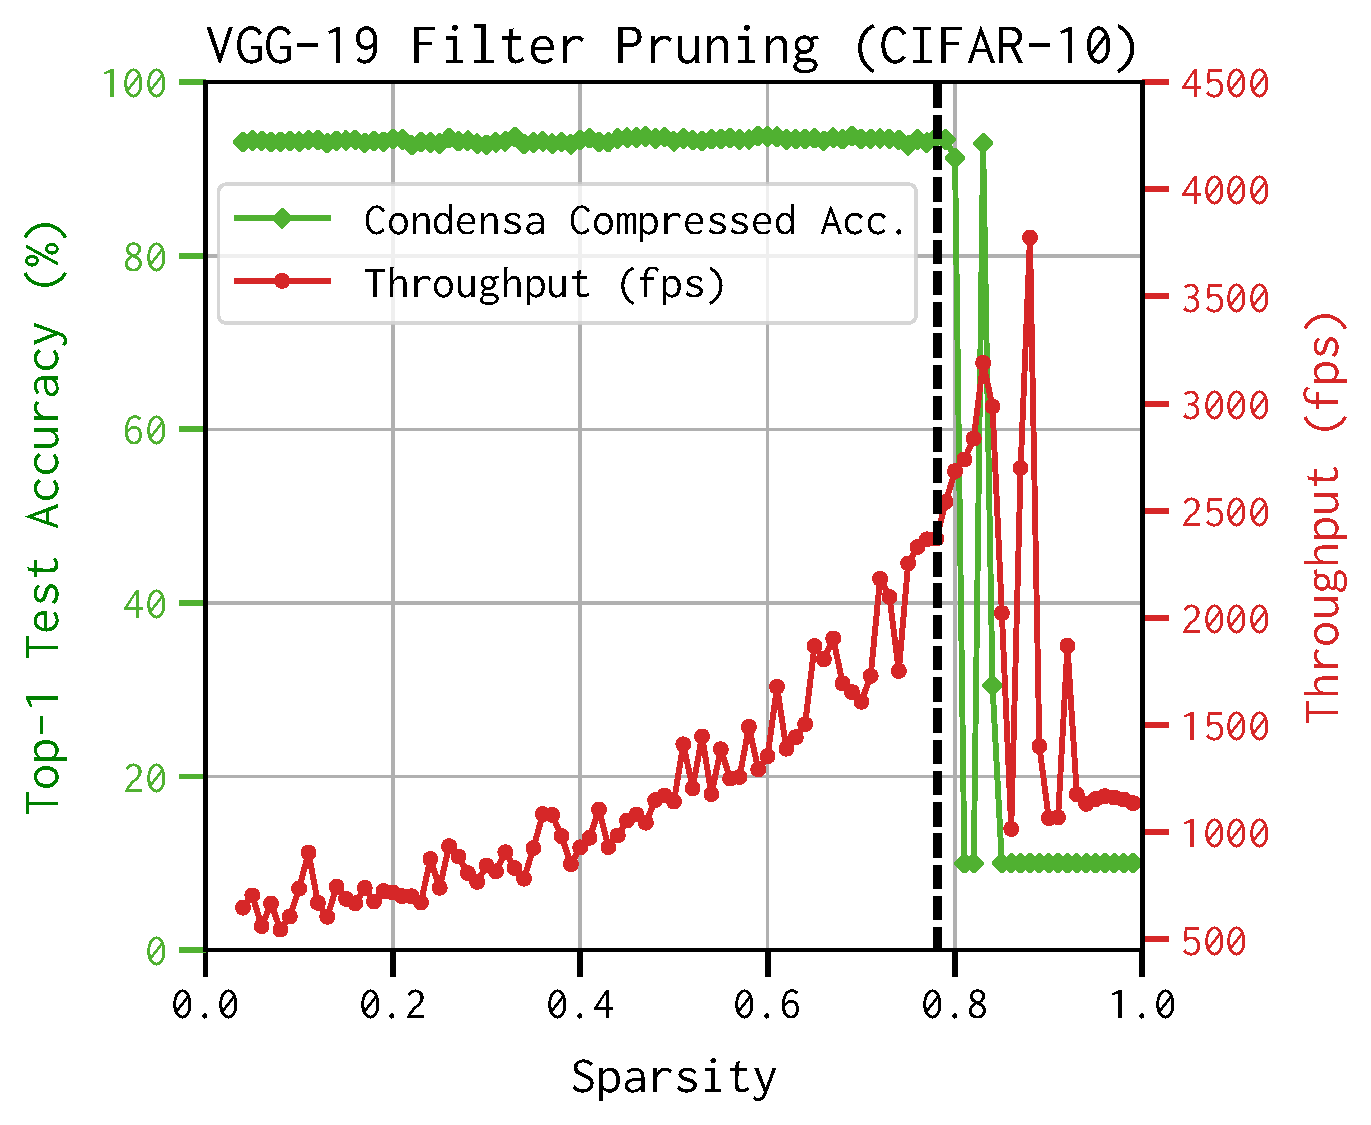
\includegraphics[width=0.5\linewidth]{img/vgg19_bn_filter_intro_v2.pdf}
%\vspace{-10pt}
\caption{Top-1 test accuracy (green) and throughput (red) vs.\ sparsity for VGG-19 on CIFAR-10.
\algoName is designed to solve constrained optimization problems of the form ``maximize throughput, with a lower bound on accuracy". In this case, \algoName automatically discovers a sparsity (vertical dashed line) and compresses the model to this sparsity,
improving throughput by $2.59\times$ and accuracy by $0.36\%$.
}
\vspace{-10pt}
\label{fig:vgg-intro}
\end{figure}

%Current approaches to model compression
%also require manual specification of compression hyperparameters, such
%as the target sparsity ratio, which is the proportion of zero-valued parameters in %the
%compressed model vs.\ the original.
%
Current approaches to model compression
also require manual specification of compression hyperparameters, such
as {\bf target sparsity}---{\em the proportion of zero-valued parameters in the
compressed model vs.\ the original.}
%
However, with current approaches, finding the best sparsity 
often becomes a trial-and-error search, with
each such trial having a huge cost (often multiple days for large models such as BERT) and involving training the compressed model to convergence,
only to find (in most cases) that the compression objectives are not met.
%
The main difficulty faced by such unguided approaches is
that sparsities 
vary unpredictably with changes in the compression context,
making it very difficult to provide users with any guidelines, whatsoever.
%
Therefore, automatic and {\em sample-efficient} approaches that minimize the number of trials are crucial
to support the needs of designers who must adapt
a variety of neural networks to a broad spectrum of platforms targeting a wide
range of tasks.

To address the above-mentioned problems of flexible expression of compression strategies, automated compression hyperparameter inference, and sample efficiency, we introduce \algoName, a new framework for programmable model compression.
\begin{figure*}[tbp]
\centering
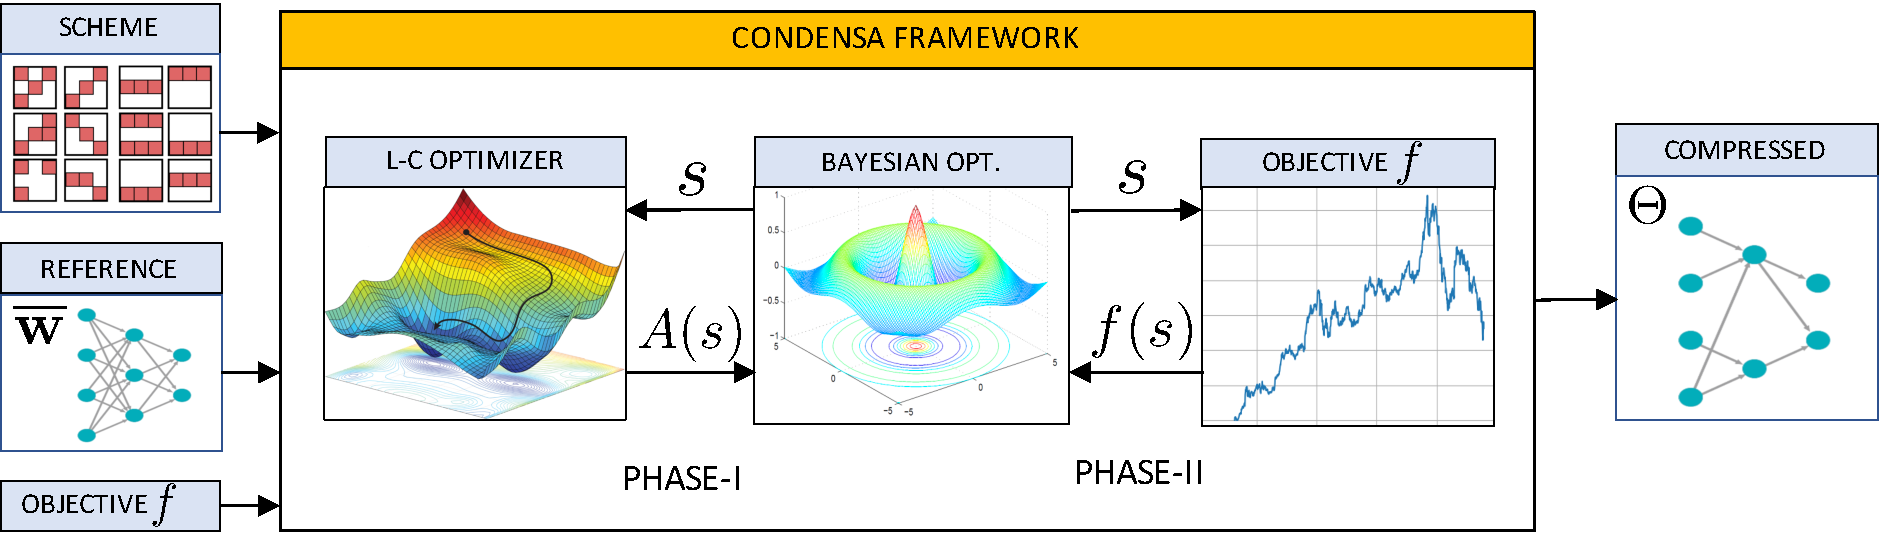
\includegraphics[width=\textwidth]{img/Overview_R4.pdf}
\caption{\algoName framework overview. The user provides the pre-trained model ($\overline{\bw}$), a compression scheme, and an objective function $f$. \algoName uses the Bayesian and L-C optimizers to infer an optimal target sparsity $s^*$ and corresponding compressed model $\Theta$.}
\label{fig:condensa}  
\end{figure*}

\begin{figure}[tb]
	\lstinputlisting[label=code:condensa,caption={Example usage of the \algoName library.}]{code/condensa.py}
\end{figure}

\begin{table}[tb]
\centering
        \begin{tabularx}{\linewidth}{ l  X }
				\hline
				\textbf{Scheme} & \textbf{Description} \\ \hline
				\texttt{Quantize(dtype)} & Quantizes network weights to given datatype \texttt{dtype}. \\ \hline
				\texttt{Prune()} & Performs unstructured pruning of network weights. \\ \hline
                \texttt{NeuronPrune(criteria)} & Aggregates and prunes neurons (1D blocks) according to \texttt{criteria}.\\ \hline
				\texttt{FilterPrune(criteria)} & Aggregates and prunes filters (3D blocks) according to \texttt{criteria}. \\ \hline
				\texttt{StructurePrune(criteria)} & Combines neuron and filter pruning.\\ \hline
				\texttt{BlockPrune(criteria, bs)} & Aggregates and prunes n-D blocks of size \texttt{bs} according to \texttt{criteria}.\\ \hline
				\texttt{Compose(slist)} & Composes together all schemes in \texttt{slist}.\\ \hline
           \end{tabularx}
	\caption{List of pre-built compression schemes in \algoName.}
	\label{tab:schemes}
\end{table}


As an illustration of the level of automation provided by \algoName,
consider the problem of improving the
inference throughput of VGG-19~\cite{simonyan2014very} on the CIFAR-10 image
classification task~\cite{krizhevsky2014cifar}.
%
Since VGG-19 is a convolutional neural network, one way to improve its
inference performance on modern hardware such as GPUs is by pruning
away individual convolutional filters~\cite{he2018progressive}.
%
Figure~\ref{fig:vgg-intro} shows the accuracy and throughput obtained
by \algoName on this task.
%
Here, we plot the compressed model's top-1 test accuracy and throughput as a function of the sparsity (green and red lines,
respectively).\footnote{Note that these curves are not known a priori and
are often extremely expensive to sample;
they are only plotted here to better place the obtained solution in context.}
%
\algoName's solution corresponds to a sparsity of $0.79$
and is depicted as the vertical dashed line.
%
This result is significant for two reasons: (1) using the \algoName library,
the filter pruning strategy employed for this experiment was expressed in
less than 10 lines of Python code, and (2) the optimal sparsity of
$0.79$ that
achieves throughput and top-1 accuracy improvements of $2.59\times$ and $0.36\%$, respectively,
was obtained automatically by \algoName using a sample-efficient constrained
Bayesian optimization algorithm.
%
Here, the user didn't have to specify any
sparsities manually, and instead only had to define a domain-specific
objective function to maximize (inference throughput, in this case).

%%%%%%%%%%%%%%%%%%%%%%%%%%%%%%%%%%%%%%%%%%%%%%%%%%%%%%%%%%%%%%%%%%%%%%%%%%%%%%%%%%%%%%%%%
%%%%% CIE
%%%%%%%%%%%%%%%%%%%%%%%%%%%%%%%%%%%%%%%%%%%%%%%%%%%%%%%%%%%%%%%%%%%%%%%%%%%%%%%%%%%%%%%%%

 Now, an increasing number of applications, including autonomous driving~\cite{teslacrash17}, surveillance~\cite{yang2018low}, and voice assistance systems~\cite{alam2020survey}, demand ML models that can be deployed on low-power and low-resource devices, and typically have strong latency requirements \cite{dennis2020edgeml, kusupati2018fastgrnn}. In such applications, the notion of {\em model compression} has gained popularity; at a high level, model compression involves taking a {\em reference model} and producing a {\em compressed model} that is lightweight in terms of computational requirements, while being functionally equivalent to the reference model (i.e., produces the same classification outputs on all inputs).
Model compression has been studied extensively in computer vision as well as other domains~\cite{cheng2017survey}, leveraging techniques such as 
structured 
weight pruning~\cite{wang2019structured,mccarley2020structured,frankle2018lottery, luo2017thinet,dong2017more,molchanov2016pruning}, quantization~\cite{zhu2016trained, gong2014compressing} and 
low-rank factorization~\cite{kossaifi2020factorized,lebedev2014speeding, , , }. 
% These individual compression schemes as well as their combinations can be expressed together in programmable compression systems such as~\cite{joseph2019condensa}. %and these individual compression
% %schemes for pruning and quantization and their interesting combinations can be expressed in \algoName and all these schemes are but some of the methods used for this task. 
% \sscmt{This violates double-blind and makes it evident that the authors are the same. I would suggest to not mention the name Condensa at all since we never used it explicitly for the final experiments.}
%
Many of these methods rely on making structural modifications to the network and then fine-tuning to potentially regain some of the accuracy loss.

However, in spite of its power and potential, model compression techniques are known to have drawbacks~\cite{8711062}. For example, certain classes may be unfairly affected in terms of classification accuracy compared to others; this may lead to unfair outcomes, e.g., ethnicity-based discrimination in facial~\cite{chekanov2017evaluating} or speech recognition~\cite{buolamwini2018gender}.
%
Mitigating this impact of compression is particularly
urgent, given the widespread use of compressed deep 
neural networks in resource-constrained and sensitive 
domains such as 
%
%
%
health care diagnostics~\cite{xie2019automated, %(Xie et al., 2019; 
gruetzemacher20183d,    %Gruetzemacher et al., 2018; 
badgeley2019deep,       %$Badgeley et al., 2019;
oakden2020hidden},       %Oakden-Rayner et al., 2019),
%
%
self-driving cars~\cite{teslacrash17}, %(NHTSA, 2017)
%
facial recognition software~\cite{
buolamwini2018gender% Buolamwini
 % Gebru, 2018b). 
}, and
%
human-resource management~\cite{amazon18, 
yourface19}. % Harwell2019
%
%
For these tasks, the trade-offs incurred by 
compression will be intolerable given the huge impact 
on human welfare.

Another class of drawbacks come from complex inputs~\cite{kendall2017uncertainties,wilmanski2016complex}, e.g., in an image with different components, the reference model may `focus' on certain aspects/features while the compressed one may focus on others. 
These drawbacks may be attributed to the fact that network compression is usually performed with the goal of simply matching the overall accuracy of the reference model. This leads us to the following question: {\em can  compression schemes ensure that the compressed and reference networks are close at a semantic or feature level?}
This question is challenging because networks can have different number of layers, features per layer and different connectivity structures. Moreover, the answer generally depends on the architecture of the reference network and the task at hand. The goal of our paper is to use ideas from knowledge distillation (such as logit pairing~\cite{ba2014do, hinton2015distilling}) to introduce new terms into the objective function of a compression scheme and help answer the above question. With new loss terms, the challenge now is to understand the relative importance of the terms and measure the impact they have on the overall objective.
%how to measure the impact of adding new terms into the objective. 

\paragraph{Compression Impacted Exemplars (CIEs)} To measure the impact of compression, we use a metric proposed in a series of work by Hooker et al.~\cite{hooker2020characterising}: counting the number of classification mismatches between the reference and the compressed model.\footnote{\label{footnote:cie-cie}Note that~\cite{hooker2020characterising} used the slightly different name of Compression {\em Identified} Exemplars; our modification is done to ensure compatibility with a similar notation for segmentation that we will define later.} This number can be {\em more informative than purely the accuracy} of the compressed model. For example, a lot of research has focused on making models more unbiased, more fair and more robust. If we have a reference model obtained using such methods, we would wish to have compression methods to preserve these properties. In fact, we consider a subset of CIEs (which we call \textit{CIE-Us} and report both CIE and \textit{CIE-U} numbers.

\begin{figure*}[!t]
\centering
  % \includegraphics[width=0.8\textwidth,height=10cm]{CVPR2021/img/FinalIntroFigure.pdf}
  \includegraphics[width=\textwidth]{img/FinalIntroFigure.pdf}
  \caption{Overview of our CIE reduction framework using label preservation-aware loss functions.}
  \label{fig:overview}
\end{figure*}

%\end{refsection}
\section{Thesis Statement}
Model compression is a ubiquitous tool that brings the power of modern deep learning 
to edge devices with power and latency constraints. The goal of model compression is 
to take a large reference neural network and output a smaller and less expensive 
compressed network that is functionally equivalent to the reference. Compression 
typically involves pruning and/or quantization, followed by executing accuracy recovery 
algorithms to maintain the reference accuracy. However, we observed that 
compression leads to a considerable mismatch in the labels produced by the reference and 
the compressed models, resulting in bias and unreliability. 
To combat this, In this thesis  we present user programmable systems for resource efficient 
model compression and methods to improve its reliability so that it can also be used for mission-critical  domains.
%\begin{refsection}
\section{Research Work}

\subsection{Condensa: A Programmable Approach to Neural Network Compression}
\subsubsection{Background, Related Work}

For a given task such as image classification, assume we have trained a large {\em reference} model $\overline{\bw} = \argmin_{\bw} L(\bw)$, where $L()$ denotes a {\em loss function} (e.g., cross-entropy on a given training set), and $\bw \in \mathbb{R}^P$. {\em Model compression} refers to finding a smaller model $\Theta$ that can be applied to the same task and ideally achieves the same accuracy as $\overline{\bw}$.
Model compression can be performed in various ways, and \algoName currently supports two commonly used techniques: pruning and quantization. In pruning, non-zero values from $\overline{\bw}$ are eliminated or ``pruned'' to obtain $\Theta$. Pruning is usually performed using some kind of thresholding (for eg., magnitude-based) and can be unstructured (prune any non-zero value) or structured (prune only {\em blocks} of non-zeros). On the other hand, quantization retains the number of parameters in $\Theta$ but assigns parameters in $\overline{\bw}$ one of K codebook values, where the codebook may be fixed or adaptive. \algoName supports low-precision approximation, which refers to assigning each parameter in $\overline{\bw}$ a corresponding lower-precision representation (for example, converting from 32-bit to 16-bit floating-point) and is equivalent to quantization using a fixed codebook.


\noindent \textbf{DNN Compression Techniques}
There is considerable prior work on accelerating neural networks using structured 
weight pruning~\cite{wang2019structured,mccarley2020structured,frankle2018lottery, han2015learning, luo2017thinet, han2017ese, dong2017more, han2016eie, polyak2015channel, hu2016network, anwar2016compact, molchanov2016pruning}, quantization~\cite{zhu2016trained, gong2014compressing} and 
low-rank tensor factorization~\cite{kossaifi2020factorized,lebedev2014speeding, xue2013restructuring, denton2014exploiting, girshick2015fast}.
Most of these individual compression
schemes for pruning and quantization and their combinations can be expressed in \algoName. Two common problems with these existing methods are: (1) determining optimal sparsity at a global (network) level, and (2) distributing global sparsity into per-layer sparsities.
We tackle these problems efficiently and systematically using our Bayesian and L-C optimizers, respectively.

\noindent \textbf{Automated Model Compression}
\begin{comment}
Bayesian optimization has previously been demonstrated to work well for general hyperparameter optimization in machine learning and neural architecture search~\cite{snoek2012practical,dai2019chamnet}.
To the best of our knowledge, we are the first to use sample-efficient search via Bayesian optimization for obtaining compression hyperparameters.
Automation in model compression is currently achieved either through reinforcement learning (RL) algorithms~\cite{he2018amc} or simulated annealing~\cite{liu2019autoslim}. 
In particular, the automation procedure for AMC~\cite{he2018amc} uses four arbitrary stages of pruning and re-training for RL training; additionally, the reward function is difficult to design, and even given a good reward, local optima can be hard to escape. It is also difficult to determine when such methods may just be overfitting to irrelevant patterns in the environment. Even disregarding generalization issues, AMC's agent (DDPG) uses trial and error, which is characterized to have an underlying incompatibility with the target pruning problem \cite{liu2019autoslim}.
AutoSlim~\cite{liu2019autoslim} proposes an automated approach based on simulated annealing, and uses the ADMM algorithm for accuracy recovery, which is an AL-based method very similar to the L-C algorithm; AutoSlim, however, only supports weight pruning and does not support general compression schemes as \algoName does. 
\end{comment}
Automating model compression involves finding both an optimal compression strategy for a given $\overline{\bw}$, along with its corresponding compression hyperparameters such as target sparsity with minimal manual intervention. Current state-of-the-art frameworks in this domain include AMC~\cite{he2018amc} and AutoCompress~\cite{liu2019autoslim}, which use reinforcement learning and simulated annealing, respectively, to automatically find desirable target sparsities for a fixed pruning strategy. \algoName, in contrast, supports the programmable expression of a wide variety of compression strategies (not just pruning). Also, in the context of automated model compression, each sample corresponds to training the compressed model to convergence, and can be extremely expensive to compute; unfortunately, techniques such as reinforcement learning, which is used in AMC~\cite{he2018amc}, can be highly sample-inefficient~\cite{mnih2013playing}. To minimize the number of samples drawn, \algoName uses a novel and sample-efficient Bayesian optimization-based algorithm for automatically arriving at desirable target sparsities. While Bayesian optimization has previously been demonstrated to work well for general hyperparameter optimization in machine learning and neural architecture search~\cite{snoek2012practical,dai2019chamnet}.
To the best of our knowledge, we are the first to use sample-efficient search via Bayesian optimization for obtaining compression hyperparameters.
%

\noindent \textbf{General Compression Algorithms and Tools} General accuracy recovery algorithms capable of handling a wide variety of compression techniques provide the foundation for systems like \algoName. Apart from the L-C algorithm~\cite{carreira2017model} which \algoName uses, other recent accuracy recovery algorithms have been proposed. ADAM-ADMM~\cite{zhang2018adam} proposes a unified framework for structured weight pruning based on ADMM that performs dynamic regularization in which the regularization target is updated in each iteration. DCP~\cite{zhuang2018discrimination} introduces additional losses into the network to increase the discriminative power of intermediate layers and select the most discriminative channels for each layer by considering the additional loss and the reconstruction error. \algoName can readily support such algorithms as additional optimizers. Neural network distiller~\cite{neta_zmora_2018_1297430}, TensorFlow model optimization toolkit~\cite{tftoolkit} {\color{black} and NNCF~\cite{kozlov2020neural} are three recent open-source model compression frameworks that support multiple compression schemes.} While these projects share a number of common goals with \algoName, they differ in two important ways: first, they do not support the expression of schemes as imperative programs containing control-flow, iteration, recursion, etc.~(Distiller requires a declarative compression specification in YAML, while the TensorFlow model optimization toolkit operates by modifying the DNN computation graph directly); second, these frameworks do not support automatic compression hyperparameter optimization for black-box objective functions.

\subsubsection{Contribution}

\begin{enumerate}
    \item It presents \algoName, a new framework for programmable neural network compression. \algoName supports the expression of
the overall compression strategy in Python using operators provided by its compression library. 
%
Since each strategy is a Python function, users are  
able to programmatically compose elementary schemes to build much
more complex and practically interesting schemes.

\item It presents a novel sample-efficient algorithm based on Bayesian optimization (B.O.) in \algoName for automatically inferring optimal sparsities based on a user-provided objective function. Given \algoName's ability to support the expression of meaningful high-level
objective functions---for example, the throughput (images/sec) of a convolutional neural network---users
are freed from the burden of having to specify compression hyperparameters manually.

\item It demonstrates the effectiveness of \algoName on three image classification and language modeling tasks, resulting in memory footprint reductions of up to $188\times$ and runtime throughput improvements of up to $2.59\times$ using at most 10 samples per search.
\end{enumerate}
\subsection{Sample Efficient Methods for Compression-Hyperparameter Search}
\subsubsection{Background, Related Work}

\paragraph{Bayesian Optimization for Hyper-Parameter Selection}
%
The process of determining the global sparsity ratio for DNN Model Compression can be viewed as an Hyper-parameter selection problem, in that view 
there are several works that approach this problem using Bayesian Optimization.
%
\cite{snoek2012practical} presented methods for performing Bayesian optimization for hyperparameter selection of general machine learning algorithms and they introduced a fully Bayesian treatment for Expected Improvement (EI), and algorithms for dealing with variable time regimes and running experiments in parallel. 
%
The effectiveness of their
approaches were demonstrated on three challenging recently published problems spanning different areas of machine learning. 
%
The resulting Bayesian optimization finds better hyperparameters significantly faster than the approaches \cite{cirecsan2012multi} used by the authors and surpasses a human expert at selecting hyperparameters on the competitive CIFAR-10 dataset, beating the state of the art by over $3\%$.

It is intuitive to split the problem of finding optimal target sparsities into two stages: (1) find the highest target sparsity that loses at most $\epsilon$ accuracy w.r.t the original uncompressed model $\overline{\bw}$, and (2) in a constrained sparsity regime obtained from stage (1), optimize a user-provided objective function $f$ (e.g., throughput, or memory footprint) and return the solution as the final sparsity.
For both stages, \algoName utilizes Bayesian optimization as shown in Figure~\ref{fig:condensa}.

Bayesian Optimization (B.O.) is an optimization framework based on continually updating a {\em probabilistic model} with measurements of a function to be optimized~\cite{jones1998efficient}. Given a set of parameters to be optimized, B.O. makes black-box calls to the objective, updates the probabilistic model with the new information, and selects the next point to evaluate using an {\em acquisition function} that combines information about the expectation and uncertainty of a function value under the probabilistic model.
\algoName employs a Gaussian Process (G.P.) model for B.O. due to its favorable statistical and computational characteristics~\cite{srinivas2009gaussian}. 
It is worth highlighting that B.O. leverages principled Bayesian inference to trade off exploration and exploitation, and is sample-efficient for non-convex black-box functions such as the ones optimized by \algoName
\cite{jones1998efficient}.

\begin{comment}
It is intuitive to split the problem of finding optimal sparsity ratios into two stages: (1) find the highest sparsity value that loses at most $\epsilon$ accuracy w.r.t the original uncompressed model, and (2) in a constrained sparsity regime obtained from stage I, optimize a user-provided objective function $f$ (e.g., throughput, or memory footprint) and return the solution as the final sparsity ratio. 

It is worth noting that optimizing performance characteristics (accuracy, throughput, and so on) against sparsity ratios requires access to function $f$, and often assumes cheap function evaluation. However, for compression, each function evaluation may amount to optimizing the full model, which is computationally prohibitive.

\algoName leverages black box sample-efficient Bayesian optimization to optimize objective $f$ with accuracy constraints. Bayesian optimization solves for the minimum of a black-box function $f(\bx)$ on some bounded set $\mathcal{X}$, which we take to be a subset of $\mathbb{R}^{D}$~\cite{mockus1978application,jones2001taxonomy}. These methods construct a probabilistic model of $f$ with sequential evaluation, and then exploit this model for sequential selection of information gathering actions---the choice of $x\in \mathcal{X}$. This procedure leverages all function evaluations instead of only local gradient approximations, and hence is sample efficient even for non-convex black-box functions~\cite{brochu2010tutorial}.


A Bayesian optimization algorithm requires two design choices: a prior and an acquisition function. The prior captures assumptions about smoothness and continuity of function $f$, while the acquisition function expresses a utility function over the model posterior for sequential decisions. 

% ====================
% \subsection{Gaussian Process Optimization}% ====================
\noindent \textbf{Gaussian Process Prior.}
The Gaussian Process (GP) is a computationally convenient prior distribution on functions that allows for closed-form marginal and conditional computations~\cite{rasmussen2006gaussian}. The GP is defined by the property that any finite set of $N$ points $\{\bx_{n} \in \mathcal{X}\}_{n=1}^{N}$ induces a multivariate Gaussian distribution on ${\mathbb{R}}^{N}$.
We assume that the function $f(x)$ is drawn from a GP prior and that our observations are of the form $\{\bx_n, y_n\}_{n=1}^{N}$, where $y_n \sim \mathcal{N}(f(\bx_n),\nu)$ and $\nu$ is the variance of noise introduced into the function observations.
The support and properties of the resulting distribution on functions are determined by a mean function $m: \mathcal{X} \rightarrow \mathbb{R}$ and a positive definite covariance function $K: \mathcal{X} \times \mathcal{X} \rightarrow \mathbb{R}$.


\noindent \textbf{Design of Acquisition Function.}
The GP prior and sequential function evaluations induce a posterior over the function of interest $f$; the acquisition function, which we denote by $a:\mathcal{X} \rightarrow \mathbb{R}^{+}$ is the utility model that guides the next best point for function evaluation.  These acquisition functions depend on the previous observations $\{\bx_n,y_n\}$ and the GP hyperparameters $\rho$; we denote this dependence as $a(\bx; \{\bx_n, y_n\}, \rho)$. 
%
Under the Gaussian process prior, the acquisition function depends on the model solely through its predictive mean function $\mu(\bx; \{\bx_n,y_n\}, \rho)$ and predictive variance function $\sigma^2(\bx; \{\bx_n, y_n\}, \rho)$.
%
For this discussion, we denote the best current value as $\bx_{\text{next}} = \text{argmin}_{\bx_n} f(\bx_n)$ and the cumulative distribution function of the standard normal as $\Phi(\cdot)$.
The choice of acquisition function depends on the overall problem objective, as illustrated following.  
%

\noindent \textit{1. Probability of Improvement}. This  intuitive strategy maximizes the probability of improving over the best current value \cite{kushner1964new}. Under the GP this can be computed analytically as: 
$a_{\text{PI}}(\bx; \{\bx_n, y_n\}, \rho) = \Phi(\gamma(\bx))$, where 
$\gamma(\bx) = \frac{f(\bx_{\text{best}}) - \mu(\bx; \{\bx_n, y_n\}, \rho)}{\sigma(\bx; \{\bx_n, y_n\}, \rho)}$.
%

\noindent \textit{2. Expected Improvement}.  Alternatively, one could choose to maximize the expected improvement (EI) over the current best.
This also has closed form under the Gaussian process:
$a_{\text{EI}}(\bx; \{\bx_n, y_n\}, \rho) = \sigma(x; \{\bx_n, y_n\}, \rho) - \kappa \sigma(\bx; \{\bx_n, y_n\}, \rho)$, with a tunable $\kappa$ to balance exploitation against exploration.
%

\noindent \textit{3. Upper/Lower Confidence Bound}. 
Here, the functional approximation uncertainty is leveraged for acquisition through lower (upper) confidence bounds for functional min (max)~\cite{srinivas2009gaussian}.
These acquisition functions have the form $a_{\text{UCB}}(\bx;\{\bx_n, y_n\};\rho) = \mu(\bx; \{\bx_n, y_{n}\}, \rho) - \kappa \sigma(\bx; \{\bx_n, y_n\}, \rho)$, with a tunable $\kappa$ to balance exploitation against exploration.

\noindent \textit{4. Level-Set Optimization}. 
    In addition to unconstrained optimization, to enable \algoName to achieve constraint satisfaction we build on top of level-set black-box optimization~\cite{bogunovic2016truncated,garg2016tumor,zanette2018robust}.
    We leverage a Gaussian Process Adaptive Sampling criterion called Implicit Level Set Upper Confidence Bound (ILS-UCB)~\cite{garg2016tumor}, that prioritizes sampling near a level set of the estimate. 
This algorithm prioritizes searching the expected L-C curve intersection with user accuracy constraints, conditional on estimated uncertainty, and does not seek to precisely learn the shape of the entire L-C curve.
Intuitively, by reducing the estimation space to specifically localize the sparsity that meets user accuracy constraints, we can reduce the total number of measurements-and consequently the time required to achieve an optimal value for the sparsity.
Hence, rather than prioritizing both high variance and high mean like UCB, ILS-UCB prioritizes sampling in areas near a level set of the mean represented by the Gaussian Process Implicit Surface, i.e. to minimize the implicit potential defined by $\mu(\bx) - L$, and where the confidence interval is large:%
%\vspace{-3pt}
\begin{equation}
\bx_t = \underset{\bx \in X}{\text{argmax}}~(1 - \gamma) \sigma(\bx) - \gamma | \mu(\bx) - L|
\label{eq:ils}
% \vspace{-2pt}
\end{equation}

\end{comment}

In \algoName's two-stage optimization pipeline, we first find a sparsity $s_{acc}$ that constrains the model accuracy function $A$ to the provided $\epsilon$. We then constrain the {\em sparsity search space} to $(0, s_{acc})$ while optimizing the user-provided objective function $f$. Note that we assume that $A$ decreases monotonically w.r.t. sparsity in the region $(0, s_{acc})$.
For each stage, \algoName uses a distinct acquisition function
to guide the next best point for function evaluation.
%It depends on the previous observations $\{\bs_n,y_n\}$ and the G.P. hyperparameters $\rho$; we denote this dependence as $AcqFn(\bs; \{\bs_n, y_n\}, \rho)$. The next sparsity to sample is given by $\bs_{\text{next}} = \text{argmax}_{\bs_n} AcqFn(\bs_n)$.

\paragraph{Stage 1: Solving Accuracy Constraints}
Recall that in the first stage of the sparsity inference process, we aim to find the highest sparsity $s_{acc}$ that loses at most $\epsilon$ accuracy w.r.t. the original reference model $\overline{\bw}$. To this end, we first define a {\em Level-Set} $L$ that represents $Acc(\overline{\bw}) - \epsilon$ and aim to find the point on the accuracy curve of the compressed model that intersects with $L$; the sparsity corresponding to this solution will be $s_{acc}$. We propose a novel acquisition function to find $s_{acc}$ named Domain-Restricted Upper Confidence Bound (DR-UCB).

DR-UCB builds upon an existing level-set black-box optimization technique named ILS-UCB~\cite{garg2016tumor}, %which is defined as follows: $\bs_{next} = \underset{\bs_{n}}{\text{argmax}}~(1 - \gamma) \sigma(\bs) - \gamma | \mu(\bs) - L|$, where $\gamma$ is a tunable hyper-parameter that controls exploration vs. exploitation. ILS-UCB
which is characterized by two properties: (1) it prioritizes searching in the region where the level set intersects the accuracy curve, (2) it does not seek to precisely learn the shape of the entire accuracy curve. However, in \algoName, since accuracy values can be safely assumed to decrease monotonically with increasing sparsity, we notice that it is also possible to progressively restrict the search domain of sparsities based on whether the currently sampled point meets the level-set constraints. In DR-UCB, we exploit this property to greatly improve sample efficiency over ILS-UCB. Mathematically, we define $\bs_t$, the sparsity value sampled at iteration $t$ using DR-UCB, as follows:
\begin{multline}
\bs_t = \underset{\bs_{}}{\text{argmax}}~(1 - \gamma) \sigma(\bs) - \gamma | \mu(\bs) - L|
    \text{s.t.} \quad \bs_t > \bs_{i} \quad \forall i \in [0, t-1], \quad \mathcal{B}_f(\bs_t)  \ge  L
    \label{eq:dr-ucb}
\end{multline}
Here, $\mathcal{B}_f$ represents the L-C accuracy function, and $\bs_t$ is (1) greater than all the previous sparsities $\bs_i$, and (2) satisfies the level set constraint $\mathcal{B}_f(\bs_t)  \ge  L$. We achieve this by minimizing the difference between the GP's mean curve $\mu(\bs)$ and the level set using the term $|\mu(\bs) - L|$ in (\ref{eq:dr-ucb});
the parameter $\gamma$ controls the trade-off between exploitation and exploration.
%The intution is that for all iterations $\forall i \in [0, t-1]$, the sparsity value currently sampled sparsity $(s_t)$ is greater than all the previous solutions $s_i$ \textit{and} this sparsity value $s_t$ satisfies the level set constraint $\mathcal{B}_f(\bs_t)  \ge  L$, 
%these two goals are obtained by minimizing the difference between the GP's mean curve $\mu(\bs)$ and the level set using the term $|\mu(s) - L|$ in (\ref{eq:dr-ucb}):
%
%where the $\gamma$ parameter is a trade-off parameter between the exploitation %and exploration. The domain restriction is expressed as the acceptance criteria:
%
Algorithm~\ref{alg:bo} illustrates how DR-UCB is employed to efficiently find $s_{acc}$.

\newcommand\CONDITION[2]%
  {\begin{tabular}[t]{@{}l@{}l@{}}
     #1&#2
   \end{tabular}%
  }
  
  \algdef{SE}[IF]{If}{EndIf}[1]%
  {\algorithmicif\ \CONDITION{#1}{\ \algorithmicthen}}%
  {\algorithmicend\ \algorithmicif}%
\algdef{C}[IF]{IF}{ElsIf}[1]%
  {\algorithmicelse\ \algorithmicif\ \CONDITION{#1}{\ \algorithmicthen}}

\makeatletter
\algnewcommand{\LineComment}[1]{\Statex \hskip\ALG@thistlm \(\triangleright\) #1}
\makeatother


\begin{algorithm}[tb]
  \caption{Bayesian Sparsity Inference with Domain Restriction}
  \label{alg:bo}
  \begin{minipage}{.95\columnwidth}
    \begin{algorithmic}[1]
     \Procedure{BO$_{DR-UCB}$}{$\mathcal{B}_f$, $L$, $T$}
        \LineComment{$\mathcal{B}_f$: Function to optimize}
        \LineComment{$L$: Level set}
        \LineComment{$T$: \# Iterations}
        \State \texttt{GP} $\leftarrow$    \texttt{GP-Regressor.initialize()}
        \State $s_0$ $\leftarrow$ $0$; $D$ $\leftarrow$ $(0, 1)$; $\mathbf{X}$ $\leftarrow$ $\emptyset$
        \For{$t \gets 1, 2, \ldots$ . $T-1$}
          \State{$s_t \gets$ $\texttt{argmax}_{D}\text{DR-UCB}(s|\mathbf{X}_{0:t-1})$}
          \State{$y_t \gets \mathcal{B}_f(s_t)$}
          \If{$s_t > s_{t-1}$ \textbf{and} $y_t \ge$ $L$}
              \State{$D$ $\leftarrow$ $(s_t,1)$}
          
        %   \State{
        %         \If{$s_t > s_{t-1}$ \textbf{and} $y_t \ge$ AcqFn.LevelSet}
        %         \State{AcqFn.bounds = $(s_t,1)$}
        %         \EndIf
        %   }
          \EndIf
        \State{$\mathbf{X}_{0:t} \gets \{\mathbf{X}_{0:t-1}, (s_t, y_t)\}$}
        \State{\texttt{GP.Update}($\mathbf{X}_{0:t}$)}
        \EndFor
        \State{\Return $s_{T-1}$}
      \EndProcedure
      \algstore{Condensa}
    \end{algorithmic}
  \end{minipage}
\end{algorithm}


\paragraph{Stage 2: Optimizing the User-Defined Objective} Once we find a  sparsity $s_{acc}$ that satisfies the user-provided accuracy constraints in stage 1, our next objective is to find the final sparsity $s^*$ that optimizes the user-defined objective function $f$ in the constrained sparsity domain $(0, s_{acc})$. For this, we employ the Upper and Lower Confidence Bound (UCB/LCB) acquisition functions for function maximization and minimization, respectively~\cite{srinivas2009gaussian}.

\begin{comment}

\noindent \textbf{Maximizing the acquisition function.}
\algoName uses a combination of random sampling and the L-BFGS-B
optimization method to find the maximum of the acquisition function. We first sample a few $(1e5)$ warmup  points at random,
and then run L-BFGS-B from $250$ random starting points.
To find the point at which to sample, we still need to maximize the constrained objective $u(\bx)$.
\textit{Unlike the original objective function, $u(\cdot)$ can be cheaply sampled}.
Existing works optimize the acquisition function using DIRECT \cite{jones1993lipschitzian}, a deterministic, derivative-free optimizer.
It uses the existing samples of the objective function to decide how to proceed to divide the feasible space into finer rectangles.
Other methods such as Monte Carlo and multi-start have also been used, and seem to perform reasonably well \cite{mockus1994application,lizotte2008practical}. Note that the second term in Equation~\ref{eq:ils} is negative, as we are trying to sample in locations where the distance to the level set is minimized.
To find the point at which to sample, we still need to maximize the constrained objective $u(\bx)$.
Unlike the original objective function $f$, $u(\cdot)$ can be cheaply sampled. In \algoName we use GP-UCB (GP-LCB) for function maximization (minimization) and ILS-UCB for solving constraints, as shown in Algorithm~\ref{alg:bo}.
%

\noindent \textbf{Algorithm Summary.}
We describe \algoName's two-stage optimization pipeline in Algorithm~\ref{alg:bo}. Here, we first find a sparsity value $s_{acc}$ that constrains the accuracy function $A$ to the provided $\epsilon$. We then constrain the search space to $(0, s_{acc})$ while optimizing the user-provided objective function $f$. The \texttt{BAYESOPT} function runs a Bayesian optimization loop given a target objective function $\mathcal{B}_f$ and an acquisition function. Note that we assume that $A$ decreases monotonically w.r.t. sparsity in the region $(0, s_{acc})$.

\end{comment}

\subsubsection{Contribution}

\begin{enumerate}
\item It presents a novel sample-efficient algorithm based on Bayesian optimization (B.O.) in \algoName for automatically inferring optimal sparsities based on a user-provided objective function. Given \algoName's ability to support the expression of meaningful high-level
objective functions---for example, the throughput (images/sec) of a convolutional neural network---users
are freed from the burden of having to specify compression hyperparameters manually.

\item We introduce the first framework that supports model compression based on user-defined constraints on target model accuracy, size and FLOP metrics instead of raw sparsity ratios.

\item It demonstrates the effectiveness of \algoName on three image classification and language modeling tasks, resulting in memory footprint reductions of up to $188\times$ and runtime throughput improvements of up to $2.59\times$ using at most 10 samples per search.
\end{enumerate}
\subsection{Correctness: Reliable Model Compression via Label-Preservation-Aware Loss Functions}
\subsubsection{Background, Related Work}

In this section, we provide a brief overview of recent model compression approaches, followed by a more detailed background on group sparsity-based model compression and CIE reduction.

% -- Upweighted CIEs (better way would be to only upweight CIEs which are not misclassified by the uncompressed model, but misclassified by the compressed model)
%
%\noindent \textbf{Model Compression}
%Definition
%LC-optimizers
%Rewind
%Magnitude-based
%Shortcomings of focusing on accuracy alone
\noindent \textbf{Model Compression}
Deep neural networks are heavy on computation and memory by design,
%
creating an impediment to operating these networks on resource-constrained platforms.
%
%
To alleviate this constraint, several branches of work 
have been proposed to reduce the size of an existing
neural network.
%
%
The most commonly employed approach 
is to reduce the number of weights, neurons, or layers in a 
network while maintaining approximately the same
performance~\cite{joseph2020programmable}.
%
This approach was first explored on DNNs
in early work such as~\cite{lecun1990optimal,hassibi1994optimal}.
%
%
Studies conducted by~\cite{han2015learning,han2015deep} %song han
showed that simple unstructured pruning can reduce the size
of the network by pruning unimportant connections within the 
network. However, such unstructured pruning strategies produce large sparse weight matrices that are computationally inefficient unless equipped with a specialized hardware~\cite{numenta20}.
%
%
To resolve this issue, structured pruning methods were proposed 
where entire channels are pruned simultaneously to ensure that the pruned network can be naturally accelerated on commodity hardware~\cite{li2016pruning,hu2016network,wen2016learning}. %the denseness of the weights.
%
More recently, Renda et al.~\cite{renda2020rewind} proposed the \textit{rewind} algorithm which is similar to simple fine-tuning of the network to regain the loss in accuracy incurred during the pruning step. The sparsity level of the model is updated in small steps where each step enhances the sparsity of the model followed by fine-tuning.
The two major schemes for structured pruning are either based on filter pruning~\cite{joseph2019condensa} or low-rank tensor factorization~\cite{li2020group}. Both these approaches enable direct acceleration of the networks in contrast to unstructured pruning.
Li et al.~\cite{li2020group} explored the relationship between tensor factorization and general pruning methods, and proposed a unified approach based on sparsity-inducing norm which can be interpreted as both tensor factorization or direct filter pruning. By simply changing the way the sparsity regularization is enforced, filter pruning and low-rank decomposition can be derived accordingly. 
This is particularly important for the compression of popular network architectures with shortcut connections (e.g. ResNet), where filter pruning cannot deal with the last convolutional layer in a ResBlock while the low-rank decomposition methods can.

\paragraph{Accuracy Recovery Algorithms} General accuracy recovery algorithms capable of handling a wide variety of compression techniques provide the foundation for modern compression systems. Prior work in this domain includes the LC algorithm~\cite{carreira2017model}, ADAM-ADMM~\cite{zhang2018adam} and DCP~\cite{zhuang2018discrimination}. More recently,
%like \algoName. Apart from the L-C algorithm~\cite{carreira2017model} which \algoName uses, other accuracy recovery algorithms are also suitable for our \emph{label-preservation loss function} formulation, for example ADAM-ADMM~\cite{zhang2018adam} a unified framework for structured weight pruning based on ADMM that performs dynamic regularization in which the regularization target is updated in each iteration.
%and also DCP~\cite{zhuang2018discrimination} which has additional losses into the network to increase the discriminative power of intermediate layers and select the most discriminative channels for each layer by considering the additional loss and the reconstruction error. 
the \textit{Rewind}~\cite{renda2020rewind} and Group-Sparsity~\cite{li2020group} algorithms have been demonstrated to be state-of-the-art compression algorithms.
Due to their compression scheme-agnostic nature, we build upon these two methods in our paper to evaluate the proposed \emph{label-preservation-aware loss functions}.
%Both these formulations are independent of both the compression scheme ($\mathcal{H}$) and the compression accuracy recovery algorithm ($\mathcal{A}$) itself given that the method allows optimizing over arbitrary differentiable loss functions.
%

\paragraph{Network Distillation}
%Teacher-student learning?
%Logit Pairing
%Kannan et al. (2018)~\cite{kannan2018adversariallogit} used the idea of logit pairing between different images to .
%Knowledge distillation (Hinton)
Another branch of network compression initially proposed by \cite{hinton2015distilling}, attempts to distill knowledge from a large teacher network to a small student network. 
%attempts to reduce the size of the network by transferring the knowledge of the full network to a student network of smaller size.
%
% By employing a loss function that teaches the student network to mimic the outputs of the teacher network, a smaller network with similar performance can be obtained.
With the assumption that the knowledge captured by a network is reflected in the output probability distribution, this line of work trains the student network to mimic the probability distribution produced by the teacher network. Since the networks are trained to output one-hot distribution, a temperature $T$ is used to diffuse the probability mass.
%
Advanced methods of distillation have succeeded in achieving much more effective transfer by not only
transferring the output logits but the information of the intermediate activations as in~\cite{zagoruyko2016paying, romero2014fitnets, jang2019learning, ahn2019variational}.
Although network distillation was presented as a general form of logit pairing, it is quite difficult to obtain improvements during distillation without spending considerable effort in manually tuning the temperature $T$ for the softmax layer. In contrast, using pure logit pairing comes without any additional cost of manual hyperparameter tuning.
Therefore, we employ pure logit pairing instead of knowledge distillation in our approach.


%
% loss function learning
% ref https://arxiv.org/pdf/1912.12355.pdf
% SoftAdapt: Techniques for Adaptive Loss Weighting of 
% Neural Networks with Multi-Part Loss Functions
%

\paragraph{Group-Sparsity based Model Compression}
%\label{sec:group_sparsity}

We now briefly describe the key insight of the compression recovery algorithm that was used in our evaluation.
The main idea in the Group-Sparsity recovery algorithm \cite{li2020group} is that the filter pruning and filter decomposition seek a compact
approximation of the parameter tensors despite their different operational forms to cope with different application scenarios.
%
Consider a vectorized image patch  $\bf{x} \in \mathbb{R}^{m \times 1}$
and a group of $n$ filters $\bf{\mathcal{W}} = \{\bf{w_1}, \cdots , \bf{w_n}\} \in \mathbb{R}^{m \times n}$.
%
The pruning methods remove output channels and approximate the original output $\bf{x}^T \bf{\mathcal{W}}$ as $\bf{x}^T \bf{C}$, where $\bf{C} \in \mathbb{R}^{m \times k}$ only has
$k$ output channels. Filter decomposition methods approximate $\bf{\mathcal{W}}$ as two filters $\bf{A} \in \mathbb{R}^{m\times k}$
and $\bf{B} \in \mathbb{R}^{k \times n}$, making $\bf{AB}$
a rank $k$ approximation of $\bf{\mathcal{W}}$. 
%
Thus, both pruning and decomposition-based methods seek a compact approximation to the original network parameters, but adopt different strategies for the approximation.
%
%
The weight parameters $\bf{\mathcal{W}}$ are usually trained with some regularization 
such as weight decay to constrain the hypothesis class.
%
To get structured pruning of the filter, structured sparsity regularization 
is used to constrain the filter:
\begin{equation}
\min _{\mathcal{W}} \mathcal{L}(y, \Phi(\mathbf{x} ; \mathcal{W}))+\mu \mathcal{D}(\mathcal{W})+\lambda \mathcal{R}(\mathcal{W})
\label{eq:loss1}
\end{equation}
%
where $\mathcal{D}(\cdot)$ and $\mathcal{R}(\cdot)$ represents the weight decay and 
sparsity regularization term respectively, while $\mu$ and $\lambda$ are the regularization factors.
%
Instead of directly regularizing the matrix $\bf{\mathcal{W}}$ \cite{yoon2017combined, li2019oicsr}, we enforced group sparsity constraints by incorporating a sparsity-inducing matrix $\mathbf{A} \in \mathbb{R}^{n \times n}$, which can be converted to the filter of a $1 \times 1$ convolution layer after the original layer.
%
%
Then the original convolution of 
$Z = X \times \mathcal{W}$ becomes 
$Z = X \times (\mathcal{W} \times \mathbf{A})$.
%
To obtain a structured sparse matrix, group sparsity regularization is enforced on $\bf{A}$. Thus, the loss Eqn. \ref{eq:loss1} function becomes
%
\begin{equation}
\min _{\mathcal{W}, \mathbf{A}} \mathcal{L}(y, \Phi(\mathbf{x} ; \mathcal{W}, \mathbf{A}))+\mu \mathcal{D}(\mathcal{W})+\lambda \mathcal{R}(\mathbf{A})
\label{eq:loss2}
\end{equation}
%
Solving the problem in Eqn. \ref{eq:loss2} results in structured group
sparsity in matrix $\textbf{A}$. By considering matrix $\bf{\mathcal{W}}$ and $\bf{A}$ together, the actual effect is that the original convolutional
filter is compressed.

\paragraph{Compression Impacted Exemplars (CIEs)}

Top-1 accuracy is just one among many possible ways of characterizing the quality of a compressed model. An alternative approach involves counting all the inputs for which the compressed model disagrees with the original, uncompressed model. Each such input is termed a {\em Compression Impacted Exemplar (CIE)}, following the definition by Hooker et al.~\cite{hooker2020characterising} (see also footnote~\ref{footnote:cie-cie}). %\sscmt{But Sara's definition was Compression Identified Exemplar. I think we should mention this explicitly without just saying that we follow the definition of Hooker et al. since this slightly deviates from it.}
While CIE reduction is critical in domains which require compressed models to match the original model as closely as possible,
we observe that reducing label mismatches is all the more important {\em when the reference model makes a correct prediction}. We term such CIEs {\em CIE-U}. We explore novel loss formulations that target both CIE and CIE-U reduction during compression.

%we observe that CIEs can be of two kinds, each with very different characteristics:

%\begin{itemize}
%    \item \textbf{CIE-C:} A CIE which the compressed model gets right (w.r.t. ground truth) but the uncompressed model gets wrong.
%    \item \textbf{CIE-U:} A CIE which the uncompressed model gets right (w.r.t. ground truth) but the compressed model gets wrong.
%\end{itemize}

%While reducing both types of CIEs is desirable for cases where the compressed model must match the reference model as closely as possible, note that there may be domains which care more about reducing CIE-Us alone (i.e., if the reference model makes a correct prediction, ensure that the compressed one does too). In Section~\ref{sec:losses}, we explore novel loss formulations to reduce the different types of CIEs subject to such constraints.
%We notice that reducing the number of CIE-Cs can {\em hamper} the performance of the final model, and that an effective CIE reduction algorithm must focus on reducing CIE-Us instead.

CIE reduction has received relatively little attention from the research community, with recent work by Hooker et al.~\cite{hooker2020characterising} being the only one that we are aware of that tries to identify and reduce CIEs. Their primary approach  involves re-weighting CIEs, where they consider a mitigation strategy of fine-tuning the compressed model for a certain number (chosen to be 3000) of iterations while up-weighting the CIEs relative
to the rest of the dataset. Their approach is sensitive to hyperparameters such as: (1) choice of number of fine-tuning iterations, (2) a threshold (90th percentile) to upweight all exemplars above that threshold, and (3) an upweighting value of $\lambda > 1$ for CIE which they choose to be $2$. We believe that our approach  is more principled for a number of reasons. First, we pose CIE mitigation as a general \emph{label-preservation} problem and extensively explore several loss functions to mitigate this without introducing any new hyperparameters than were initially used during model compression or changing any of the values of the original compression hyperparameters. Lastly, we are agnostic to the compression scheme and compression algorithm.

%In Section~\ref{sec:losses}, we introduce novel loss functions that are specifically designed to reduce total CIEs and CIE-Us without adversely affecting CIE-Cs. 
%\noindent Minimizing the disagreement between the two models in the first case will hamper it's performance on the data, which is undesirable. Therefore, minimization only in the second case is desirable. In order to circumvent this problem, we again introduce the cross-entropy loss into the picture, but in conjunction with the logit pairing loss.




\paragraph{Multi-Part Loss Functions} 
% soft-adapt
% Recently more work is being done on how loss functions affect learning 
Networks that perform challenging tasks or multiple 
tasks often require a combination of losses to work. Considerable effort has been made towards understanding the role of different loss terms~\cite{huang2019addressing,barron2019general,chen2018gradnorm}, and how best to combine them. 
%
%
% Multiple losses are typically combined by taking an 
% equally-weighted linear combination of
% each objective function; but the importance of each part
% could be different and thus components should be assigned...
% weights as per their contribution to the learning. 
While most of the prior work combines these losses either using ad-hoc or equal weights, %. However, the actual contribution of each loss is difficult to manually compute. The weights of different loss functions can even vary over the training time where some losses can be useful to initially bootstrap the model while some are useful in gaining an extra performance boost towards the end of the training cycle.
%
% On the other hand, the scaling of each component of the 
% loss function can inhibit the ability of the optimizer 
% by only looking at loss components with the largest magnitude.
% ...
%In recent years, the need for weighting the components
%of multi-part functions has become more evident, and 
researchers have recently tried to develop systematic methods to adjust
the weights on the linear combination of loss components.
%
%
These methods often require defining new loss functions~\cite{barron2019general} or changing the optimization procedure~\cite{chen2018gradnorm}. %, but there is limited research on the formulation of a general method
%that can be added to existing architectures. 
%
%
%In most cases, the integration with the current models requires sophisticated adjustment or much longer computation time.
As we describe in Section~\ref{sec:loss_opti}, we compare three different hyperparameter tuning strategies to optimize our multi-part loss function.

\subsubsection{Contribution}

\begin{itemize}
    \item Employing additional loss terms in the compression objective based on the teacher-student paradigm so as to align the predictions of the reference and the compressed models. %logit pairing term into the network compression objective, thus exploiting the teacher-student learning paradigm along with a term for aligning the predictions of the reference and compressed models. \sscmt{Both of these are the same. Do you mean aligning predictions of the compressed model and the actual targets?} 
    We show for the first time that such a pairing can be extended to other tasks, by considering semantic segmentation. Figure~\ref{fig:motivation} shows an example of the effect of the different loss terms on the number of model mismatches.
    \item Analyzing automated strategies for tuning the hyperparameters associated with our multi-part loss functions. We demonstrate that our framework is robust to the choice of tuning strategies, and uniform weighting works as well as more intricate strategies across different datasets and reference network architectures.
    \item Through extensive experiments, we validate the effectiveness of our framework and show that it not only improves metrics such as the number of CIEs, but also yields better compression accuracy compared to previous approaches. %\sscmt{perhaps we should mention that it's mainly due to the fact that we further decompose CIEs into CIEs-U and CIEs-C, and optimize not to align the logits in cases where the prediction of the reference model is wrong}. 
\end{itemize}

% What is a good way to design a label-preservation optimization formulation
% Trying to be Agnostic to Compression Recovery Algorithms.

While the teacher-student paradigm is a coarse way to capture ``semantic similarity'' between the reference and compressed models, our results show that it can nonetheless be highly effective in reducing the number of CIEs.
We also remark that our methodology can work with any compression scheme that allows us to specify a custom objective that can be optimized to produce a compressed model. 

%\end{refsection}
\section{Remaining Work and Timeline}

 \renewcommand*{\thefootnote}{\fnsymbol{footnote}}
 \setcounter{footnote}{1}
 \footnotetext{Non-Thesis Work}
 \renewcommand*{\thefootnote}{\arabic{footnote}}
 \setcounter{footnote}{0}

\begin{table*}[h]
\centering
\begin{center}
%\begin{scriptsize}
\begin{sc}
\begin{tabular}{ll}
\toprule
\textbf{Papers\textsuperscript{$\checkmark$} Patents\textsuperscript{$\dagger$} and Presentations\textsuperscript{$\ddagger$}}                                                  & \textbf{Timeline}        \\ \midrule
Effective Paralleization of Belief Propation on the GPU\textsuperscript{$\ddagger$} .\footnotemark                  & NVIDIA GTC 2018          \\ 
Message scheduling for performant, many-core belief propagation\textsuperscript{$\checkmark$} .\footnotemark[1]         & IEEE HPEC 2019           \\ \midrule
A Programming System and Automation Libraries for Model Compression\textsuperscript{$\checkmark \ddagger$}                           & Baylearn-19, NeurIPS-19, GTC-19 \\
Model Compression for Health care Devices: Challenges and Opportunities\textsuperscript{$\ddagger$}    & GE HealthCare 2019       \\
A Programmable Approach for Neural Network  Compression\textsuperscript{$\checkmark$}                  & IEEE MICRO 2020          \\
Bayesian Optimization for Model Compression\textsuperscript{$\dagger$}                              & NVIDIA 2019              \\ \midrule
Correctness-preserving Compression of Datasets and Neural Networks\textsuperscript{$\checkmark$} & Correctness SC 2020      \\
Reliable Model Compression via Label-Preservation-Aware Loss Functions\textsuperscript{$\checkmark$}   & CVPR 2020 (Under Review) \\
Mitigating the Bias \& Attribution Problems for Fairness \& Safety\textsuperscript{$\checkmark$} & KDD 2021 (Proposed Venue)                             \\ \midrule
\textbf{Dissertation Defense}                                            & \textbf{Spring 2021} \\   
\bottomrule
\end{tabular}
\label{tab:results}
  \end{sc}
%\end{scriptsize}
\end{center}
\end{table*}

\subsection{Class-wise CIEs: Mitigating The Bias problem for Fairness in Edge Inference}
The most black-box way to understand a network is to study the classification it provides for different input classes.  This does not tell us how the network arrives at the classification, but it contains more fine-grained information than the aggregate accuracy.  Figure~\ref{fig:r56Output-class-wise} illustrates 
%\ggcmtside{Move "Impact of ResNete56... from being a title to the caption. Also label the Y axis. Also merge with Figure 4 -- or maybe not!}
how a state-of-the-art compression tool~\cite{joseph2019programmable} affects the error in certain classes more significantly than others --- something we wish to avoid as it may result in unfair treatment~\cite{hooker2019selective}. 

\begin{figure}[!h]
    %\begin{minipage}[t]{0.55\linewidth}
    \centering
    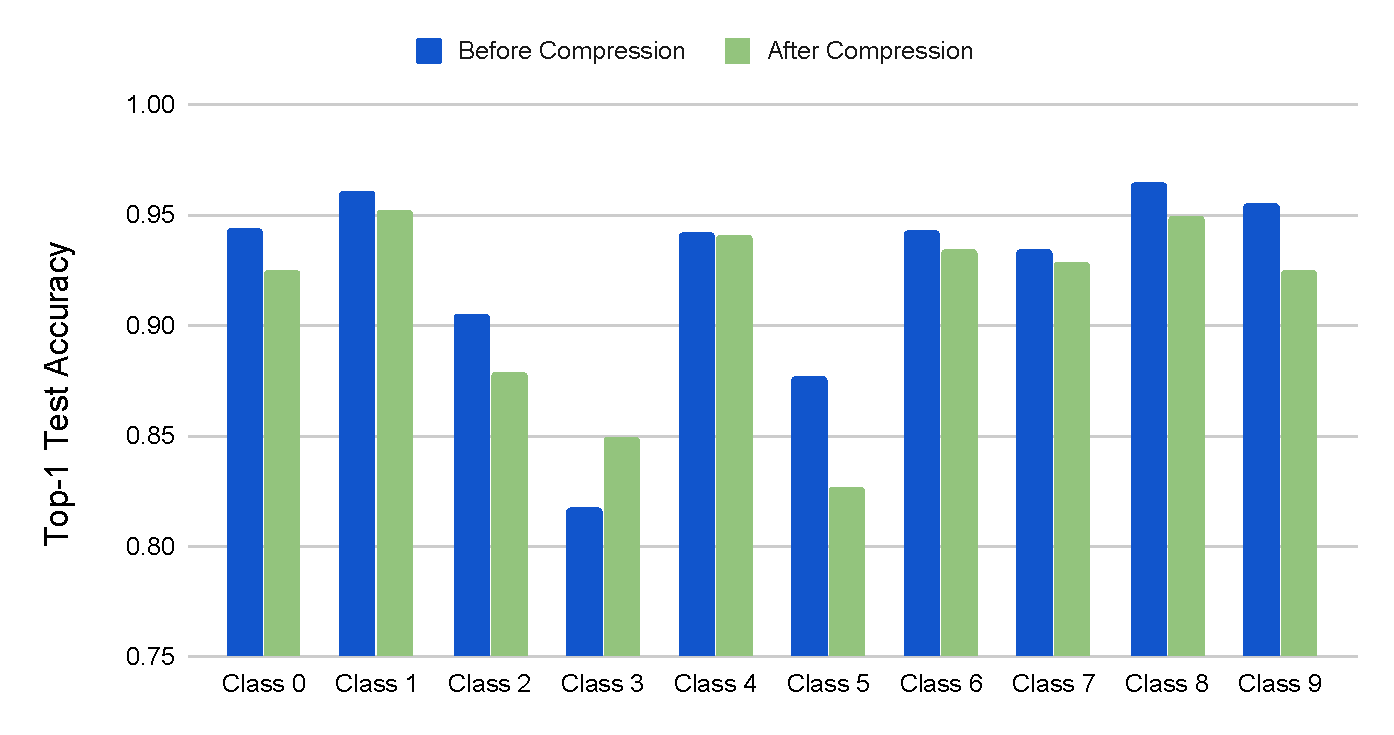
\includegraphics[width=\linewidth,clip,trim=0 .25in 0 0]{img/class-impact.pdf}
    %\vspace{-0.2in}
    \caption{\small Effect of compression on class-wise accuracy (CIFAR-10 with ResNet56 architecture)}
    \label{fig:r56Output-class-wise}
    %\end{minipage}%
\end{figure}

While class-wise accuracy numbers are more nuanced than the overall accuracy, they are still a coarse representation of the underlying issues. For example, we often observe ``structure'' in the misclassifications: some classes are much more likely to be misclassified as a few other classes than the rest of the classes.  That is, compression may result in one mammal being misclassified as another mammal, but very rarely as an object. This distinction can be important for safety and security, and depending on the application (e.g., autonomous driving, home cameras), some misclassifications are more costly than others. We capture this distinction using an application-specific metric or a distance function $d(y_1,y_2)$ between classes $y_1$ and $y_2$ (see~\cite{qin2018verification}). Denoting the reference and the compressed networks by $f$ and $\widetilde{f}$ respectively (these are functions mapping the inputs $\bx$ to labels $y$), the total misclassification cost of $\widetilde{f}$ relative to $f$ is
\[ \Delta_{\mu, d}(\widetilde{f}, f) :=  \sum_{\bx} \mu (\bx) d(\widetilde{f}(\bx), f(\bx)),\]
where $\mu(\bx)$ is the weight of the input $\bx$.  The main questions we study are, \textit{(1)} how do known compression algorithms perform with respect to the above metric for different choices of $d$ and the reference network? \textit{(2)} how can we incorporate this metric into the compression procedure?\label{tmc-measure}
%

Answering the first question will lead to an understanding of which compression scheme is better for a given application. Also, it may suggest that some reference networks are more compressible than others while maintaining semantic information. Such trends have been observed in our current framework ~\cite{joseph2019programmable}. 
%\ggcmtside{Is this where to refer to this figure? It was not referenced before. I also made up the caption. Check it.} 
%
Answers to the second question will lead us to
better domain-specific compression. 
%
Given a metric $d$ and weights $\mu$, the \ardent{} system will allow a user to optimize the standard training loss, while incorporating constraints on $\Delta_{\mu, d}$.  To achieve this, we need a notion of the derivative of the distance $d$, which provides a direction for changing $\widetilde{f}$ that reduces the objective. One natural way to define this is to make $\widetilde{f}(\bx)$ move towards $f(\bx)$.  But depending on the structure of the metric $d$, better definitions are possible. To illustrate, if an image $\bx$ of a husky is misclassified as a chair, it may suffice (for certain applications) to move $\widetilde{f}(\bx)$ towards one of the dog classes, and not necessarily a husky. This weaker requirement could lead to better compression.  \ardent{} will allow ways to specify $d$ that allow such optimization, including hierarchical metrics (cf.~\cite{Babenko2009SimilarityMF,Bengio2010Label}) and metrics 
where the class labels are embedded in a Euclidean space.\label{hier-metrics}

\subsection{Attribution Matching for Sensitive Edge Inference Tasks}

\paragraph{Motivation}
Mitigating the impact of compression is particularly
urgent given the widespread use of compressed deep 
neural networks in resource constrained but sensitive 
domains such as 
%
%
%
health care diagnostics 
\cite{xie2019automated, %(Xie et al., 2019; 
gruetzemacher20183d,    %Gruetzemacher et al., 2018; 
badgeley2019deep,       %$Badgeley et al., 2019;
oakden2020hidden}       %Oakden-Rayner et al., 2019),
%
%
,self-driving cars 
\cite{teslacrash17} %(NHTSA, 2017)
%
facial recognition software
\cite{
buolamwini2018gender% Buolamwini
 % Gebru, 2018b). 
} and
%
hiring
\cite{amazon18, 
yourface19}.% Harwell2019
%
%
For these tasks, the trade-offs incurred by 
compression will be intolerable given the huge impact 
on human welfare.
%
Due to the success of Deep learning, there is an 
emergent trend to utilize deep neural networks (DNNs) 
even for safety-critical applications such as 
self-driving cars and health-care applications 
\cite{estava2017dermatologist,
samala2018evolutionary, lane2018deep}.
%
Due to the inherent nature of such devices, 
it is of paramount importance that the utilized 
DNNs be reliable and trustworthy to human users.
%

For a system to be reliable, perpetual service 
must be rendered and the integrity of the system 
must hold even under unexpected circumstances.
%
%
For most commercially deployed DNNs, this condition 
is hardly met as they are often operated in the 
cloud due to their heavy computational requirements.
%
%
However, this dependence on clouds acts as a 
critical weakness in safety-sensitive settings 
as intermittent communication failuers to the 
cloud may cause difficulties in reacting to 
situations immediately, or even-worse, 
the device's connection to the cloud may be 
severed indefinitely.
%
%
Thus, to guarantee reliable service, 
the DNNs must be embedded on the edge device.
%
%
%
To this end, network compression techniques such 
as pruning \cite{han2015deep,li2016pruning} and distillation \cite{hinton2015distilling,zagoruyko2016paying} 
are commonly employed - as a compressed network 
would require less computational time and memory 
but maintain its prediction performance to a 
certain acceptable margin, effectively substituting 
the original network for edge computation.
\begin{figure}[!h]
    \centering
    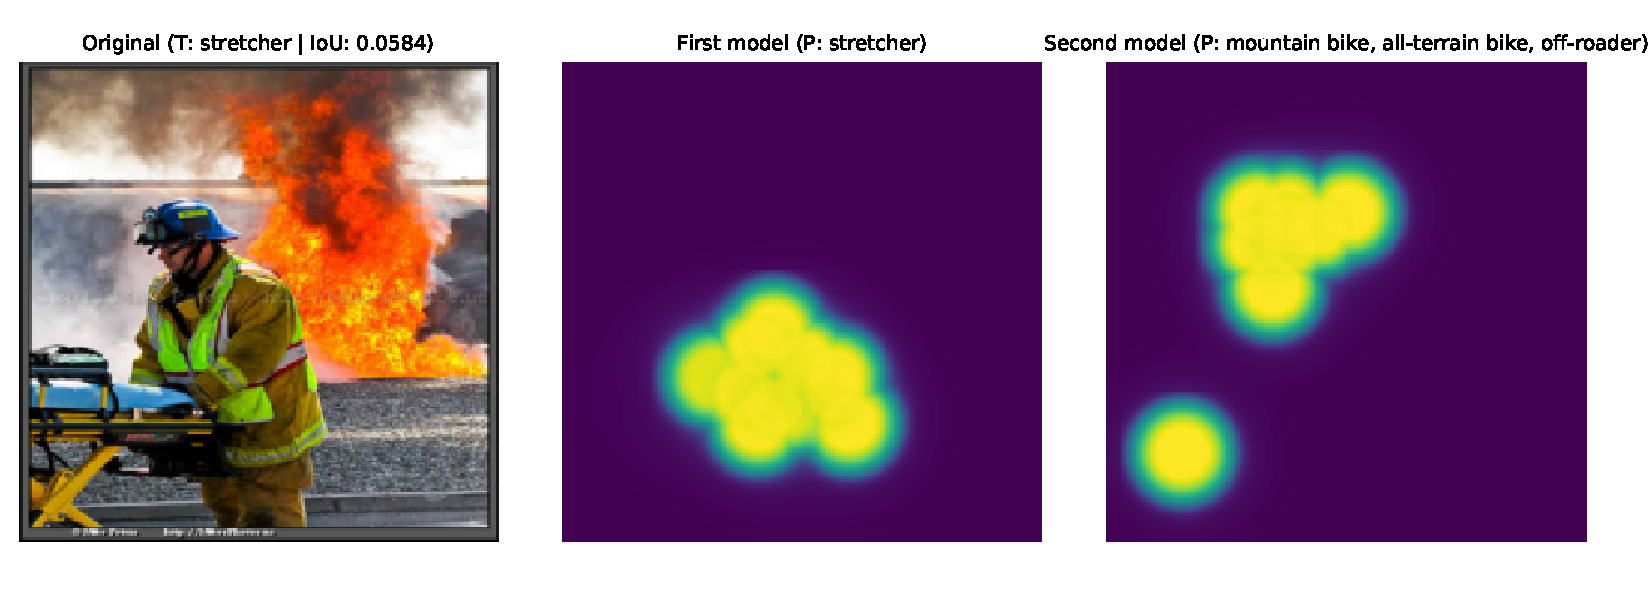
\includegraphics[width=\linewidth]{img/fire.pdf}
    %\vspace{-0.2in}
    \caption{\small Image from ImageNet's \textit{stretcher} class, along with saliency maps showing the parts of the image ``most responsible'' for classification by the reference and compressed models. Former obtains the correct class, while the latter classifies as {\em mountain bike, all-terrain bike}.}
    \label{fig:fire}
    %\vspace{-0.2in}
\end{figure}
At the same time, for a system to be trustworthy, 
the system must be transparent enough for humans 
to understand its workings and the reasons for its outputs.
%
%
An example would be when a health monitor 
predicts an onset of disease \cite{xu2019current}
- then the clinician would require an acceptable
explanation to the device output.
%
%
However, the black-box nature of deep neural 
networks complicates this goal - impeding its 
advance in safety-critical areas.
%
%
For DNNs to gain trustworthiness, the ability 
to explain why the network makes such decisions 
is essential. Such field of interest - 
eXplainable AI (XAI) - has emerged as one of the 
importance frontiers in the field of deep learning.
%
%
Amoung numerous XAI methods, the most commonly 
used methods are attribution methods \cite{selvaraju2017grad}, 
which weigh the parts of the input data according to 
how much they 'contributed' to produce the output prediction.
%
%
Such attribution methods are beginning to be applied
in safety-critical fields \cite{liang2020prediction}.

To ensure the safety of the system, 
the two aforementioned conditions should be simultaneously 
satisfied - the embedded DNNs must be equipped with 
both compression and attribution.
%
%
However we show for the first time that these seemingly
unrelated techniques conflict with each other:
compressing a network causes deformations in 
the produced attributions, even if the predictions 
of the network stays the same before and after compression.
%
%
This is a potentially severe crack in the 
integrity of the compressed network, 
as the premise in which a compressed network 
is acceptable in safety-critical fields is that 
the compressed network in as reliable as its former self.
%
%
\textit{This implies that the compressed nework must behave 
almost identically to the pre-compression network while being
smaller in size.}
%
%
Moreover, the classifications between the network are
not only different from their past counterparts 
but also broken down compared to their respective ground truths
%
%
\begin{itemize}
    \item Examples where the compressed model gets the example 
          right but the uncompressed model gets it wrong.
    \item Examples where the uncompressed model gets it right 
          but the compressed model gets it wrong.
\end{itemize}
%
%
These label distortions directly
cause incorrect interpretations, which could lead to dire 
consequences for safety-critical systems.
%
%
Such a problem arises from the pitfall of existing 
network compression approaches: they only
aim to maintain the prediction quality of the network while 
reducing the size of the network.
%
%
Compressing a network forces the network to cram its 
necessary decision procedures and information inside a
smaller space.
%
This space restriction forces the network to abandon its 
standard decision procedures and resort to using shortcuts 
and hints that are seemingly indecipherable to humans.
%
Thus, its decision procedures would become harder to 
interpret, which is reflected in its production of deformed
attribution maps
%
%
To resolve this newfound unintended
issue, we propose a novel label-preservation aware 
compression framework  to ensure both the reliability and 
trustworthiness of the compressed model.
%
...we concentrate on the observation that the labels 
of the pre-network (teacher) are closer to the ground truth signal 
compared to the post-network (student).
%
Thus, in the absence of ground truth signals, the labels
of the teacher can serve as a proxy. 
%
In this sense, we propose a automatically parameter 
tuned regularizer learning framework that matches the 
of the now-compressing network to its attribution maps 
before compression, transferring the attributional power 
of the pre-network to the post-network. Our work sheds 
new light on transfer learning techniques from the perspective of XAI,
as they can be re-interpreted and subsumed under our framework.

In many safety-critical
applications,
  one may have constraints  
  such as
  ``{\sl the two networks focus on the same aspects of an image},'' or 
  ``{\sl certain aspects of an image are not used for classification}.''  To incorporate such constraints, we propose the using methods from interpretability research such as saliency maps and influence attribution~\cite{SimonyanVZ13,fergus2013Visualizing,Kim2018Interpretability,Mukund2017Axiomatic}.
  %\ggcmtside{Give a one-sentence definition of influence attribution?} 
  These techniques give a way to ``trace'' the factors in an input that contributed to the overall classification.  Given a network and an input image $\bx$, a method such as~\cite{Mukund2017Axiomatic,Kim2018Interpretability} outputs the influence (or attribution score) of each pixel on the overall classification.

Interestingly, we find that in many cases of discrepancy between the reference and the compressed model (e.g., Figure~\ref{fig:fire}), the attributions differ significantly, indicating that the two models focus on different regions of the input.  Given the attribution scores $\alpha$ and $\alpha'$, we consider the weighted Jaccard similarity (a generalization of the natural {\em intersection-over-union} (IoU)) metric:%\ggcmtside{Cite IoU, ensure reviewer feels included.}
\[ \text{sim}(\alpha, \alpha') = \frac{ \sum_i \min( \alpha_i, \alpha'_i )}{\sum_i \max (\alpha_i, \alpha'_i) }. \]
When deploying a compressed network, a natural goal is to have high value for this similarity.  This can help avoid possible security issues during deployment,
 and in general lead to a higher agreement between the models.
\label{fse-metric}
%One reason is that the reference network may have been carefully trained to avoid specific biases (e.g. skin color), and we do not want the compression procedure to introduce bias. Another (informal) reason is that a high similarity score implies that both networks are using the {\em same features} of an image, which makes them more likely to agree on the classification.
\algoName will support incorporating the $\text{sim}()$ objective during compression, and moreover, this will be done for a range of attribution methods (including but not limited to~\cite{SimonyanVZ13,Mukund2017Axiomatic,ancona2018towards}).

\renewcommand\refname{\vskip -1cm}
\section{References}
\bibliographystyle{abbrv}
\printbibliography

\end{document}

%%% Local Variables:
%%% mode: latex
%%% TeX-master: "root"
%%% End:
